\scanpage{69}
% archive sheet number: 68

$E$ over $K$, equipped with a $\handwritten{\sigma}$-linear \deleted{endomor} \uline{automorphism} $F_E$\handwritten{;} \deleted{\unsure{$E\quad E$}} which it is useful to interpret as a $K$-li\unsure{\'{n}|\deleted{e}n}\unsure{\deleted{a}e|\deleted{e}a}\unsure{\deleted{i}a|\deleted{a}i}r isomorphism
\[
F_E : E^{\handwritten{\sigma}} = E\otimes_K(K,\handwritten{\unsure{\deleted{\sigma}\sigma|\sigma}})\handwritten{\longrightarrow} E\ .
\]
The tensor operations are defined by transport of structure (cf. case of a group, here $\underline{Z}$, acting on a field ....). The effective F-isocrystals are then interpreted as the $(E,F_E)$ such that $F_E$ leaves invariant \unsure{\deleted{in}a|\deleted{a}in} lattice, which also means that the set of iterates $F_E^n$, $n\handwritten{\geqslant}0$, is \uline{bounded} in \unsure{the|the}\deleted{\unsure{x}} vector space $\operatorname{End}(E)$. Every$(E,F_E)$ becomes \inserted{obviously}\handwritten{\begin{tikzpicture}[x=1cm,y=1cm,baseline=-.1cm]\draw[thin] (0,.15).. controls (.05,-.1) and (-.2,-.1)..(-1,-.1).. controls (-1.3,-.1) and (-1.6,-.2)..(-1.6,-.5);\end{tikzpicture}} effective after multiplication of $F_E$ by a suitable power of $p$, which is another way of saying that the category of F-iso\unsure{\deleted{v}c|\deleted{c}v|w}rystals is obtained from that of effective F-\deleted{si}\handwritten{is}ocrystals \deleted{by} by making $K\handwritten{(}-1)$ \unsure{\deleted{e}i|\deleted{i}e}nvertible .

\handwritten{4.} The Tannakian category $\mathrm{Fcriso}(k)$ is an interesting arith\inserted{\handwritten{m}}\handwritten{\begin{tikzpicture}[x=1cm,y=1cm,baseline=-.1cm]\draw[thin] (-.1,-.4).. controls (0,0) and (.15,.15)..(.4,.4);\end{tikzpicture}}etic invariant attached to $k$ (functorially); \deleted{specification} knowledge of it is equivalent to that of the associated gerbe (over $\underline{Q}_p$), say $\underline{G}(k)$\handwritten{\unsure{?|;|.}} Among the additional structures which should be studied at the same time as this gerb\unsure{\deleted{r}e|\deleted{e}r|e}, one must include the effectivity structure of the category $\mathrm{F}\unsure{\deleted{r}c|\deleted{c}r}\unsure{\deleted{\mathrm{ir}}\handwritten{\mathrm{ri}}|\handwritten{\mathrm{ri}}}\mathrm{so}(k)$ of \deleted{the} its linear representations, that \unsure{\deleted{da}of|\deleted{of}da} \deleted{\unsure{there|the}}the \deleted{F}\handwritten{T}ate object\handwritten{'}s inverse (defining a canonical homomorphism from $\underline{G}(k)$ to the trivial gerbe with group $\underline{G}_m$), finally for perfect $k$ at least, the datum of the natural fibre functor over $K(k)$ (which is therefore a section of the gerbe $\underline{G}(k)$ over $K(k)$); for non-perfect $k$, it would \deleted{nai\illegible{1}}be appropriate \deleted{to} to study likewise the section of $\underline{\unsure{\deleted{E}G|\deleted{G}E}}(k)$ over the field of fractions $K$ of any $p$-ring $W$ with residue field $k$.

The interest of the notion of \deleted{non-degenerate} F-crystal comes from the fact that one \unsure{has|has} \deleted{\unsure{not}} a ``crystalline cohomology'' functor
\[
X\handwritten{\mathrel{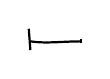
\begin{tikzpicture}[x=1cm,y=1cm,baseline=-.05cm]\draw[thick] (0,-.11)--(-.02,.16);\draw[thick] (0,0).. controls (.2,-.03) and (.4,0)..(.64,0);\draw[thick] (.64,-.025)--(.64,.025);\end{tikzpicture}}} H^{\handwritten{*}\deleted{\unsure{k|i}}}_{\mathrm{cris}}(X)
\]
